\chapter{Proofs and Experimental Results}\label{ResultsChapter}
The results of my research consist of proofs and experimental performance for the implementations described in Chapter \ref{MethodsChapter}. This chapter consists of two sections, one for generalization proofs and the other describing extraction and performance. The Kernel Perceptron generalization proofs can be found in subsection \ref{KPProofs}. Subsection \ref{KPBProofs} provides the Budget Kernel Perceptron generalization, and the Description Kernel Perceptron generalization is located in subsection \ref{KPDProofs}. In Section \ref{HaskellExtractionPerformance}, the extraction directives for the three implementations are detailed in subsection \ref{DetailsHaskellExtraction} which transform the Coq implementations to Haskell modules. Subsections \ref{SyntheticResults}, \ref{IrisResults}, \ref{SonarResults} describe the testing methodology for three datasets that were used to evaluate the experimental generalization error and analyze the runtime of training and testing each implementation. Finally, in subsection \ref{ResultsDiscussion}, the trends and results seen across datasets and implementations are outlined. The conclusions and future work for this research follow in Chapter \ref{ConclusionsChapter}.
\section{Generalization Proofs}\label{Proofs}
In the MLCert framework, much of the proof burden has been automated. For a new Learner representing a machine learning algorithm, there are two new lemmas that need to be proved. The first lemma proves the cardinality of the parameters used by the algorithm, which corresponds to the size of the parameter space. The second lemma applies the first in order to prove a generalization bound for the Learner as a whole. An example of the second lemma for a generic Learner is shown in Figure \ref{LearnerLemma}.

\begin{figure}
    \caption{Generalization Bound for a generic Learner}
    \label{LearnerLemma}
    \begin{lstlisting}
Lemma Learner_bound eps (eps_gt0 : 0 < eps) init : 
    @main A B Params Hypers Learner
      hypers m m_gt0 epochs d eps init (fun _ => 1) <=
    #|Params| * exp (-2%R * eps^2 * mR m).
    \end{lstlisting}
\end{figure}

The definition of main which is used in Figure \ref{LearnerLemma} can be found in the file ``learners.v''. Once main has been instantiated with the specifics of the Learner, such as its particular Params and Hypers, there are proofs in ``learners.v'' such as the lemma main\_bound which provide the machinery necessary to prove this inequality over the real numbers. As described by Bagnall and Stewart \cite{BS19}, MLCert uses Hoeffding's inequality, a type of Chernoff bound, to prove the generalization bound for a Learner. In the following subsections, the lemmas proving the generalization bounds for the Kernel Perceptron, Budget Kernel Perceptron, and Description Kernel Perceptron will be discussed.
\subsection{Kernel Perceptron Generalization Proofs}\label{KPProofs}
The bound for the Kernel Perceptron relies on the size of the parameter space. As proven in the lemma K\_card\_Params in the section KernelPerceptronGeneralization, the cardinality of the parameters for the Kernel Perceptron is shown in Equation \ref{KPParams}. This power of 2 is calculated by unfolding the definition of Params, which consists of the training set and a float array of size m. As all values are floating point numbers stored in 32 bits, the cardinality of a single floating point number is $2^{32}$. Therefore, as the dimensions of the training set are equal to m training examples multiplied by n dimensions, the cardinality of the training set is equal to $2^{m*n*32}$. The cardinality of a float array of size m is $2^{m * 32}$. 

\begin{equation} \label{KPParams}
 \#|Params| = 2^{(m*n*32 + m*32)}
\end{equation}

Kcard\_Params is central to the proof of the generalization bounds of the Kernel Perceptron in the lemma KPerceptron\_bound, which is defined in Figure \ref{KPLemma}. The generalization bound for the Kernel Perceptron is very loose, as growth in the size of the training set causes exponential growth in the generalization error. This limits the usefulness of the Kernel Perceptron's generalization bound, as a loose generalization bound provides few guarantees for performance or correctness. However, the Kernel Perceptron bound allows for comparison between this result and the generalization bounds for the Budget Kernel Perceptron and the Description Kernel Perceptron. 

\begin{figure}
    \caption{Generalization Bound for the Kernel Perceptron}
    \label{KPLemma}
    \begin{lstlisting}
Lemma Kperceptron_bound eps (eps_gt0 : 0 < eps) init : 
    @main A B Params KernelPerceptron.Hypers 
      (@KernelPerceptron.Learner n m KPsupport_vectors H K)
      hypers m m_gt0 epochs d eps init (fun _ => 1) <=
    2^(m*n*32 + m*32) * exp (-2%R * eps^2 * mR m).
    \end{lstlisting}
\end{figure}

\subsection{Budget Kernel Perceptron Generalization Proofs}\label{KPBProofs}
The Budget Kernel Perceptron has a similar bound on the cardinality of the parameter space. However, the parameter space for the Budget Kernel Perceptron is not dependent on m, the size of the training set, whatsoever. Instead, the parameter space relies on (S sv), which is the size of the support set. The successor of sv is used to denote the size of the support set so that the budget update procedure is always possible regardless of the value of sv, as there will be at least one support vector able to be replaced.
\\Like the Kernel Perceptron, the Budget Kernel Perceptron stores the support set and a float array. The float array is of size (S sv), so its cardinality is $2^{32 * (S sv)}$. The support set stores (S sv) training examples, which consist of one float value for each of the n dimensions of the data, plus a Boolean value for the label of the support vector. Therefore, the cardinality of each training example in the support set is $2^{1 + n * 32}$. The full cardinality of the Budget Kernel Perceptron Params is given in Equation \ref{KPBParams}. The lemma proving this bound is found in the section KernelPerceptronGeneralizationBudget, named Kcard\_Params\_Budget.

\begin{equation} \label{KPBParams}
 \#|Params| = 2^{((32*(S sv) + ((1 + n * 32)*(S sv))))}
\end{equation}

Figure \ref{KPBLemma} shows the lemma for the generalization bound of the Budget Kernel Perceptron, which uses Kcard\_Params\_Budget in its proof. Comparing the bound of the Budget Kernel Perceptron to the Kernel Perceptron, the overall structure of the two bounds is similar when the number of training examples is the same. However, because the support set can be significantly smaller than the number of training examples, the Budget Kernel Perceptron's bound is tighter than that of the base Kernel Perceptron. 

\begin{figure}
    \caption{Generalization Bound for the Budget Kernel Perceptron}
    \label{KPBLemma}
    \begin{lstlisting}
Lemma Kperceptron_bound_budget eps (eps_gt0 : 0 < eps) init : 
    @main A B Params KernelPerceptronBudget.Hypers 
      (@KernelPerceptronBudget.Learner n sv F K U)
      hypers m m_gt0 epochs d eps init (fun _ => 1) <=
    INR 2^((32*(S sv) + ((1 + n * 32)*(S sv)))) * exp (-2%R * eps^2 * mR m).
    \end{lstlisting}
\end{figure}

\subsection{Description Kernel Perceptron Generalization Proofs}\label{KPDProofs}

The generalization bound for the Description Kernel Perceptron is similar to that of the Budget Kernel Perceptron. First, we must define the cardinality of the parameter space used by the Description Kernel Perceptron. The parameters store a single float32 value paired with (S des) support vectors. The successor of des is used as the size of the support set, so that support vector replacement is always possible. Like with the Budget Kernel Perceptron, the cardinality of each support vector in the support set is $2^{1 + n * 32}$, which stores a single Boolean label as well as $n$ 32-bit floating point values. However, because there is not a float value for every support vector, only the cardinality of a single float32 must be added to the cardinality of the entire support set. The cardinality of the Description parameters is shown in Equation \ref{KPDParams}.

\begin{equation} \label{KPDParams}
 \#|Params| = 2^{((32 + ((1 + n * 32)*(S des))))}
\end{equation}

Figure \ref{KPDLemma} shows the generalization bound of the Description Kernel Perceptron in the lemma Kperceptron\_bound\_Des. This bound is similar to the bound of the Budget Kernel Perceptron, but is tighter because there is only one float32 value instead of a float32 value per support vector. This small difference means that if the budget is the same as the number of mistakes, the Description Kernel Perceptron will have a slightly tighter bound. 

\begin{figure}
    \caption{Generalization Bound for the Description Kernel Perceptron}
    \label{KPDLemma}
    \begin{lstlisting}
Lemma Kperceptron_bound_Des eps (eps_gt0 : 0 < eps) init : 
    @main A B Params KernelPerceptronDes.Hypers 
      (@KernelPerceptronDes.Learner n des F K)
      hypers m m_gt0 epochs d eps init (fun _ => 1) <=
    INR 2 ^ (32 + (1 + n * 32) * (S des)) * exp (-2%R * eps^2 * mR m).
    \end{lstlisting}
\end{figure}

\section{Haskell Extraction and Performance Experiments}\label{HaskellExtractionPerformance}
In order for the Coq implementations to be run, these implementations must be extracted to Haskell. The file ``extraction\_hs.v'' contains extraction directives for Haskell so that some Coq functions and data structures are extracted properly. The last Coq module for each implementation uses the extractible\_main definition, found in ``learners.v'', to also provide the necessary machinery that Learner.t relies on. The extracted Coq code is written to a Haskell file located in the directory hs/ in MLCert.
\\The extracted Haskell code for a machine learning algorithm does not contain code to initialize the system with training and testing data or functions to display accuracy and generalization error results to the user. Unverified Haskell drivers have been written for these implementations, which include the extracted Haskell code as a module. The Haskell drivers for the Kernel Perceptron implementations can also be found in the hs/KernelPerceptron/ directory.
\subsection{Details of Haskell Extraction}\label{DetailsHaskellExtraction}
The extraction directives for the Kernel Perceptron can be found in the section KPerceptronExtraction in the file ``kernelperceptron.v''. This section extracts the Kernel Perceptron to the Haskell file ``KPerceptron.hs'', a Haskell module that can be included by a Haskell driver program. This file is extracted to the two locations in MLCert where Haskell driver programs reside: hs/KernelPerceptron/ and hs/KernelPerceptron/timing\_drivers/. The Budget Kernel Perceptron and Description Kernel Perceptron each have their own extraction directives to extract ``KPerceptronBudget.hs'' and ``KPerceptronDes.hs'' to these same locations. 
\\There are four different kinds of Haskell driver programs for a variety of different purposes. All driver programs report the training accuracy, test accuracy, and generalization error for the dataset run by that driver. Several also print the model produced by training. The drivers are differentiated by their file names, which identify the purpose of the drivers.
\\``KPerceptronXOR.hs'' tests that the Kernel Perceptron using a quadratic kernel can classify the XOR function with 100\% accuracy. The linear kernel cannot be used because the XOR function is not linearly separable. The four samples for this function are specified in the driver, along with the quadratic kernel for the prediction function. When run, this driver demonstrates that the Kernel Perceptron behaves as expected with the quadratic kernel and is able to classify data that is not linearly separable. This is the only driver that uses nonlinear data and a nonlinear kernel function for prediction.
\\Each implementation has a driver that generates a new linearly separable dataset using a random number generator to test that the implementation can execute. These drivers have Test in their file names. After randomly generating $n$ floating point values between -1 and 1, these values form the linear hyperplane used to produce labels for the training and test examples, which are randomly generated by the same process. These synthetic datasets test that the implementations have been set up correctly and can classify linear data. However, because the datasets are generated differently for each run of the program, these drivers cannot be used to compare implementations.
\\To compare the accuracy of an implementation on a specific dataset, each implementation has a driver which reads a dataset from files and performs training and testing. These drivers have RunFile in their file names. The drivers require that the input dataset be stored in two files, one containing the training set and the other containing the test set. The dataset files must also be formatted with one example per line and values separated by commas. The first value of the line must be a positive unique integer, which is used by the Kernel Perceptron to differentiate between the training examples for updates. The last value must be either True or False, corresponding to the label for the example. As long as the dataset files are formatted correctly, the driver will train and test on this dataset and report the accuracy and generalization error for this dataset. Only one dataset is run by this driver.
\\Finally, to time the execution of training and testing on a dataset, drivers with FileIO in their name read in one or more datasets. The FileIO drivers run training and testing five times and report the time in seconds. There are a total of fifteen drivers to time all datasets, five for each implementation. The drivers do not time reading the dataset files and use the same format as the RunFile drivers. 
\\In the following subsections, I will detail my testing methodology on three datasets, two real datasets downloaded from the UCI Machine Learning Repository \cite{DG17} and a synthetic dataset created from randomly generated linear hyperplanes. The Iris Data Set \cite{Fis36} and Sonar Mines vs. Rocks Data Set \cite{SG88} were formatted to conform to be more easily read into the driver programs. Each of the following subsections describes the dataset under test, the experimental setup and drivers used, the calculated generalization error, and the timing results for training and testing.
\subsection{Synthetic Dataset Performance Results}\label{SyntheticResults}
A synthetic dataset was created specifically to test the performance of the Kernel Perceptron and its variants. There are twenty independent trials in this dataset with training and testing sets based on randomly generated data separated by a randomly oriented linear hyperplane. Each trial contains a thousand training examples and a thousand test examples, each with three dimensions. These datasets were created by recording and formatting the output of twenty runs of KPerceptronTest.hs. 
\\Because the Kernel Perceptron variants are all deterministic, the generalization error results were found using the RunFile driver for each implementation. All implementations ran for 5 epochs. The Budget Kernel Perceptron limited the size of the support set to one hundred examples, 10\% of the training set, and the Description Kernel Perceptron was similarly limited to one hundred mistakes. 
\\Generalization error results

\begin{figure}[h]\label{SyntheticGenErrFig}
 \caption{Synthetic Generalization Error}
 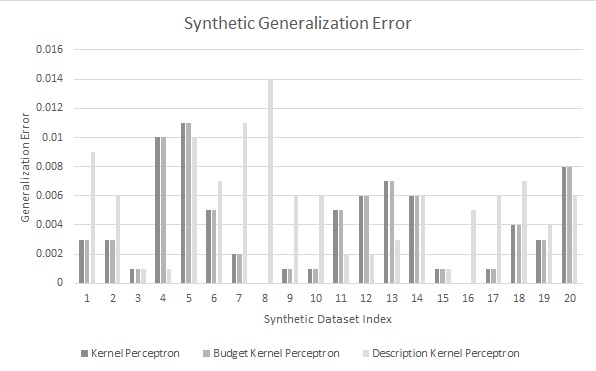
\includegraphics[scale=0.9]{SyntheticGenErr}
\end{figure}

\begin{table}[h!]
 \begin{center}
  \caption{Average Synthetic Generalization Error and Confidence Intervals}
  \label{tab:avesyntheticaccgen}
  \begin{tabular}{l|c|c|c}
  \textbf{ } & \textbf{Kernel Perceptron} & \textbf{Budget KP} & \textbf{Description KP}\\
  \hline
  \textbf{Average Training Accuracy} & 98.61\% & 98.61\% & 96.915\%\\
  \textbf{Average Testing Accuracy} & 98.58\% & 98.58\% & 96.87\%\\
  \textbf{Average Generalization Error} & 0.39\% & 0.39\% & 0.565\%\\
  \textbf{95\% Confidence Interval} & 0.001435352 & 0.001435352 & 0.001539834\\
  \end{tabular}
 \end{center}
\end{table}

\begin{table}[h!]
 \begin{center}
  \caption{Synthetic Generalization Bound Calculations}
  \label{tab:syntheticgencalc}
  \begin{tabular}{l|c|c|c}
  \textbf{ } & \textbf{Kernel Perceptron} & \textbf{Budget KP} & \textbf{Description KP}\\
  \hline
  \textbf{Training Examples} & 1000 & 1000 & 1000\\
  \textbf{Dimensionality} & 3 & 3 & 3\\
  \textbf{Support Vectors} & 1000 & 100 & 100\\
  \textbf{eps = 0} & 6.90947E+38531 & 1.93617E+3883 & 4.20647E+2929\\
  \textbf{eps = 1} & 1.78025E+37663 & 4.98862E+3014 & 1.08381E+2061\\
  \end{tabular}
 \end{center}
\end{table}

\begin{figure}[h]\label{SyntheticGenErr2Fig}
 \caption{Synthetic Generalization Error using Limited Budget and Mistakes}
 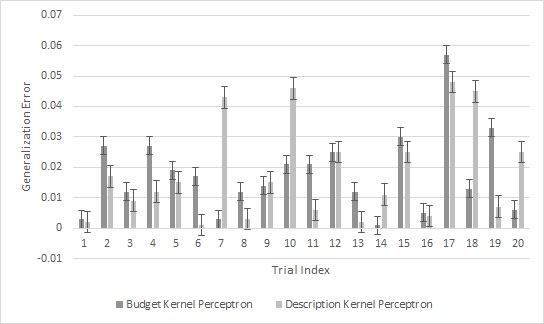
\includegraphics[scale=0.9]{SyntheticGenLimit}
\end{figure}

\begin{table}[h!]
 \begin{center}
  \caption{Synthetic Generalization Error and Confidence Intervals using Limited Budget and Mistakes}
  \label{tab:syntheticlimitedgen}
  \begin{tabular}{l|c|c}
  \textbf{ } & \textbf{Budget KP} & \textbf{Description KP}\\
  \hline
  \textbf{Training Examples} & 1000 & 1000\\
  \textbf{Dimensionality} & 3 & 3\\
  \textbf{Support Vectors} & 2 & 2\\
  \textbf{eps} & 0.301 & 0.282\\
  \hline
  \textbf{Calculated Bound} & 9.35\% & 9.10\%\\
  \textbf{Greatest Observed Generalization Error} & 5.7\% & 4.8\%\\
  \hline
  \textbf{Average Training Accuracy} & 76.89\% & 78.625\%\\
  \textbf{Average Testing Accuracy} & 76.6\% & 78.11\%\\
  \textbf{Average Generalization Error} & 1.79\% & 1.805\%\\
  \textbf{95\% Confidence Interval} & 0.005794861 & 0.007007097\\
  \end{tabular}
 \end{center}
\end{table}

Timing results

\begin{figure}[h]\label{SyntheticKernelTiming}
 \caption{Kernel Perceptron Synthetic Timing}
 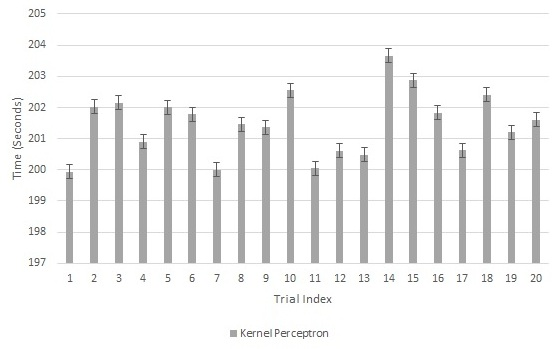
\includegraphics[scale=0.9]{KernelSyntheticTiming}
\end{figure}

\begin{figure}[h]\label{SyntheticBudgetDesTiming}
 \caption{Budget and Description Kernel Perceptron Synthetic Timing}
 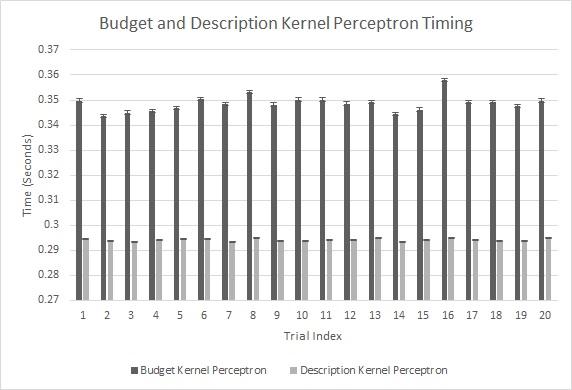
\includegraphics[scale=0.9]{BudgetDesSyntheticTiming}
\end{figure}

\begin{table}[h!]
 \begin{center}
  \caption{Synthetic Average Runtimes and Confidence Intervals}
  \label{tab:synthetictiming}
  \begin{tabular}{l|c|c|c|c|c|c}
  \textbf{Trial} & \textbf{KP} & \textbf{95\% CI} & \textbf{Budget KP} & \textbf{95\% CI} & \textbf{Description KP} & \textbf{95\% CI}\\
  \hline
  \textbf{1} & 199.943 & 3.17258 & 0.3498 & 0.05499 & 0.2946 & 0.05606\\
  \textbf{2} & 202.025 & 2.44561 & 0.3436 & 0.05116 & 0.2938 & 0.05499\\
  \textbf{3} & 202.145 & 2.78125 & 0.345 & 0.05245 & 0.2932 & 0.05529\\
  \textbf{4} & 200.901 & 2.62953 & 0.3456 & 0.05263 & 0.294 & 0.05441\\
  \textbf{5} & 202.012 & 2.97056 & 0.3468 & 0.05351 & 0.2946 & 0.05557\\
  \textbf{6} & 201.786 & 2.46189 & 0.3504 & 0.05567 & 0.2944 & 0.05666\\
  \textbf{7} & 199.996 & 2.66681 & 0.3484 & 0.05175 & 0.2934 & 0.05422\\
  \textbf{8} & 201.455 & 3.07707 & 0.3532 & 0.05527 & 0.295 & 0.05440\\
  \textbf{9} & 201.362 & 2.92524 & 0.3482 & 0.05479 & 0.2936 & 0.05558\\
  \textbf{10} & 202.546 & 2.92950 & 0.3502 & 0.05332 & 0.2938 & 0.05452\\
  \textbf{11} & 200.051 & 2.58570 & 0.3502 & 0.05332 & 0.2942 & 0.05432\\
  \textbf{12} & 200.609 & 3.10256 & 0.3486 & 0.05215 & 0.294 & 0.05537\\
  \textbf{13} & 200.479 & 3.28990 & 0.3492 & 0.05331 & 0.2948 & 0.05647\\
  \textbf{14} & 203.655 & 3.41870 & 0.3444 & 0.05226 & 0.2934 & 0.05323\\
  \textbf{15} & 202.866 & 4.18980 & 0.3462 & 0.05384 & 0.294 & 0.05489\\
  \textbf{16} & 201.827 & 3.75820 & 0.358 & 0.05232 & 0.295 & 0.05587\\
  \textbf{17} & 200.627 & 3.80374 & 0.3492 & 0.05333 & 0.2942 & 0.05528\\
  \textbf{18} & 202.409 & 3.09442 & 0.3492 & 0.05381 & 0.2938 & 0.05450\\
  \textbf{19} & 201.203 & 2.51938 & 0.3476 & 0.05410 & 0.2938 & 0.05646\\
  \textbf{20} & 201.605 & 2.93406 & 0.3498 & 0.05351 & 0.295 & 0.05442\\
  \end{tabular}
 \end{center}
\end{table}

\subsection{Iris Dataset Performance Results}\label{IrisResults}
Description of Dataset
\\Experimental setup and drivers
\\Generalization error results

\begin{table}[h!]
 \begin{center}
  \caption{Iris 50/50 Dataset Observed and Calculated Generalization Error}
  \label{tab:iris50gencalc}
  \begin{tabular}{l|c|c|c}
  \textbf{ } & \textbf{Kernel Perceptron} & \textbf{Budget KP} & \textbf{Description KP}\\
  \hline
  \textbf{Training Examples} & 77 & 77 & 77\\
  \textbf{Testing Examples} & 73 & 73 & 73\\
  \textbf{Dimensionality} & 4 & 4 & 4\\
  \textbf{Support Vectors} & 77 & 7 & 7\\
  \hline
  \textbf{Training Accuracy} & 100\% & 100\% & 100\%\\
  \textbf{Testing Accuracy} & 100\% & 100\% & 100\%\\
  \textbf{Generalization Error} & 0\% & 0\% & 0\%\\
  \hline
  \textbf{eps = 0} & 3.08721E+3036 & 6.76217E+271 & 1.07728E+214\\
  \textbf{eps = 1} & 4.05710E+2969 & 8.88660E+204 & 1.41572E+147\\
  \end{tabular}
 \end{center}
\end{table}

\begin{table}[h!]
 \begin{center}
  \caption{Iris 75/25 Dataset Observed and Calculated Generalization Error}
  \label{tab:iris75gencalc}
  \begin{tabular}{l|c|c|c}
  \textbf{ } & \textbf{Kernel Perceptron} & \textbf{Budget KP} & \textbf{Description KP}\\
  \hline
  \textbf{Training Examples} & 113 & 113 & 113\\
  \textbf{Testing Examples} & 37 & 37 & 37\\
  \textbf{Dimensionality} & 4 & 4 & 4\\
  \textbf{Support Vectors} & 113 & 11 & 11\\
  \hline
  \textbf{Training Accuracy} & 100\% & 100\% & 100\%\\
  \textbf{Testing Accuracy} & 100\% & 100\% & 100\%\\
  \textbf{Generalization Error} & 0\% & 0\% & 0\%\\
  \hline
  \textbf{eps = 0} & 4.19104E+5442 & 1.33083E+533 & 6.23051E+436\\
  \textbf{eps = 1} & 2.96325E+2969 & 9.40956E+434 & 4.40525E+338\\
  \end{tabular}
 \end{center}
\end{table}

Timing results

\begin{figure}[h]\label{IrisTiming}
 \caption{Iris Data Set Timing}
 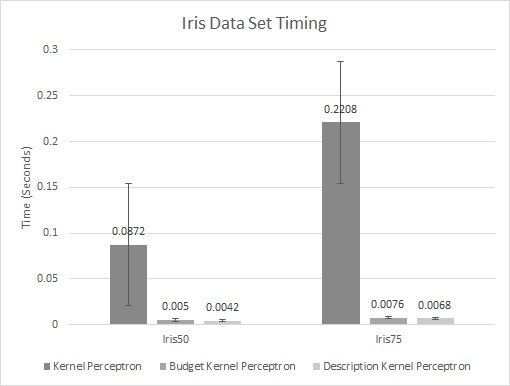
\includegraphics[scale=0.9]{IrisTiming}
\end{figure}

\begin{table}[h!]
 \begin{center}
  \caption{Iris Average Runtimes and Confidence Intervals}
  \label{tab:iristabtiming}
  \begin{tabular}{l|c|c|c|c|c|c}
  \textbf{Trial} & \textbf{KP} & \textbf{95\% CI} & \textbf{Budget KP} & \textbf{95\% CI} & \textbf{Description KP} & \textbf{95\% CI}\\
  \hline
  \textbf{Iris 50/50} & 0.0872 & 0.00342 & 0.005 & 0.00392 & 0.0042 & 0.00431\\
  \textbf{Iris 75/25} & 0.2208 & 0.00563 & 0.0076 & 0.00462 & 0.0068 & 0.00501\\
  \end{tabular}
 \end{center}
\end{table}

\subsection{Sonar Mines vs. Rocks Dataset Performance Results}\label{SonarResults}
Description of Dataset
\\Data normalization
\\Experimental setup and drivers
\\Generalization error results

\begin{table}[h!]
 \begin{center}
  \caption{Sonar 50/50 Dataset Observed and Calculated Generalization Error}
  \label{tab:sonar50gencalc}
  \begin{tabular}{l|c|c|c}
  \textbf{ } & \textbf{Kernel Perceptron} & \textbf{Budget KP} & \textbf{Description KP}\\
  \hline
  \textbf{Training Examples} & 116 & 116 & 116\\
  \textbf{Testing Examples} & 92 & 92 & 92\\
  \textbf{Dimensionality} & 60 & 60 & 60\\
  \textbf{Support Vectors} & 116 & 11 & 11\\
  \textbf{Epochs} & 10,000 & 10,000 & 10,000\\
  \hline
  \textbf{Training Accuracy} & 100\% & 55.17\% & 55.17\%\\
  \textbf{Testing Accuracy} & 69.57\% & 51.09\% & 51.09\%\\
  \textbf{Generalization Error} & 30.43\% & 4.08\% & 4.08\%\\
  \hline
  \textbf{eps = 0} & 6.66773E+68162 & 1.06512E+6467 & 4.98653E+6370\\
  \textbf{eps = 1} & Would not compute & 1.86671E+6366 & 8.73934E+6269\\
  \end{tabular}
 \end{center}
\end{table}

\begin{table}[h!]
 \begin{center}
  \caption{Sonar 75/25 Dataset Observed and Calculated Generalization Error}
  \label{tab:sonar75gencalc}
  \begin{tabular}{l|c|c|c}
  \textbf{ } & \textbf{Kernel Perceptron} & \textbf{Budget KP} & \textbf{Description KP}\\
  \hline
  \textbf{Training Examples} & 157 & 157 & 157\\
  \textbf{Testing Examples} & 51 & 51 & 51\\
  \textbf{Dimensionality} & 60 & 60 & 60\\
  \textbf{Support Vectors} & 157 & 15 & 15\\
  \textbf{Epochs} & 10,000 & 10,000 & 10,000\\
  \hline
  \textbf{Training Accuracy} & 84.08\% & 54.14\% & 54.78\%\\
  \textbf{Testing Accuracy} & 82.35\% & 50.98\% & 50.98\%\\
  \textbf{Generalization Error} & 1.73\% & 3.16\% & 3.8\%\\
  \hline
  \textbf{eps = 0} & 7.18772E+92254 & 4.71762E+8818 & 6.49060E+8683\\
  \textbf{eps = 1} & Would not compute & 2.01955E+8682 & 2.77855E+8547\\
  \end{tabular}
 \end{center}
\end{table}

Timing results

\begin{table}[h!]
 \begin{center}
  \caption{Sonar Average Runtimes and Confidence Intervals}
  \label{tab:sonartabtiming}
  \begin{tabular}{l|c|c|c|c|c|c}
  \textbf{Trial} & \textbf{KP} & \textbf{95\% CI} & \textbf{Budget KP} & \textbf{95\% CI} & \textbf{Description KP} & \textbf{95\% CI}\\
  \hline
  \textbf{Sonar 50/50} & 1045.839 & 1.49470 & 79.0278 & 2.06799 & 66.1688 & 1.28507\\
  \textbf{Sonar 75/25} & 2121.471 & 6.43889 & 138.6656 & 4.08308 & 121.6616 & 3.08207\\
  \end{tabular}
 \end{center}
\end{table}

\subsection{Discussion of Generalization Error and Timing Results}\label{ResultsDiscussion}
\section{Chapter Summary}\label{ResultsChapterSummarySection}
These results from the implementations of the Kernel Perceptron, Budget Kernel Perceptron, and Description Kernel Perceptron demonstrate that the generalization error for the Kernel Perceptron can be improved through limiting the size of the support set or placing a limit on the number of mistakes made during training. The conclusions drawn from these results are described in Chapter \ref{ConclusionsChapter}, along with a discussion of future work to be done in the field of machine learning verification.
